\documentclass{alex_hü}

\name{Alexander Helbok}
\course{PS Physik}
\hwnumber{6}

\begin{document}
	\renewcommand{\labelenumi}{\alph{enumi})}
	
	
	\section*{51. Schiefe Ebene}
	\begin{enumerate}
		\item $ M = 90 \si{\kg};\quad g = 9.81 \si{\m\per\s};\quad \alpha = \ang{35} $
		\begin{flalign*}
			F_G &=  \dl{Mg} = 883 \si{\N} &&\\
			F_{\parallel} &= F_G * \sin(\alpha) = \dl{506 \si{\N}} &&\\
			F_{\perp} &= F_G * \cos(\alpha) = \dl{723 \si{\N}} &&\\
		\end{flalign*}
		\item $ \mu_K = 0.105 $
		\begin{flalign*}
			F_{ges} &= F_{\parallel} - F_{\perp} * \mu_K = \dl{430 \si{\N}} &&\\
		\end{flalign*}
		\item
		\begin{flalign*}
			v(t) &= \dl{\tfrac{F_{ges}}{M}\ t = \tfrac{430 \si{\N}}{90 \si{\kg}}\ t} &&\\
			v(3) &= \tfrac{430 \si{\N}}{90 \si{\kg}}*3\si{\s} = \dl{14.\dot{3} \si{\m\per\s}} &&\\
		\end{flalign*}
		\item $ F_{Luft} = \tfrac{1}{2}\rho Ac_wv^2;\quad \rho = 1.293 \si{\kg\per\m^3};\quad c_w \approx 0.78;\quad A_{Aufrecht} \approx 1 \si{\m^2} $ 
		\begin{flalign*}
			F_{ges} &= F_{Luft} &&\\
			430 &= \tfrac{1}{2}*1.293*1*0.78v^2 &&\\
			v_{max} &= \sqrt{\tfrac{860}{1.293*0.78}} &&\\
			v_{max} &= \dl{29.2 \si{\m\per\s}} &&\\
		\end{flalign*}
			$ v_{max} $ ist am Zeitpunkt, wo die Summe der Kräfte in Fahrtrichtung gleich null ist (also keine Beschleunigung stattfindet), weil wenn der Schifahrer noch Beschleunigt haben wir $ v_{max} $ entweder noch nicht erreicht (Beschleunigung ist positiv) oder schon verpasst (Beschleunigung ist negativ).\\[3ex]
			$ A_{Hocke} \approx \tfrac{1}{3}A_{Aufrecht}  $
		\begin{flalign*}
			v_{max} &= \sqrt{\tfrac{860*3}{1.293*0.78}} &&\\
			v_{max} &= \dl{50.6 \si{\m\per\s}} &&\\
		\end{flalign*}
		\item 
		\begin{flalign*}
			v(t) &= 50.6 \si{\m\per\s} &&\\
			t &= \dl{10.6 \si{\s}} &&\\
		\end{flalign*}
	\end{enumerate}
	
	\section*{60. Absturz eines Fadenpendels}
	$ K = E_{Kin} = \tfrac{mv^2}{2};\quad P = E_{Pot} = mgh;\quad F_{Z} = F_{Zentripetal} = \tfrac{mv^2}{L} $
	\begin{multicols}{2}
		\begin{enumerate}
		\item \vspace{0.3cm}
		\begin{flalign*}
			E_{ges} &= mgL &&\\
			K_0 &= E_{ges} &&\\
			\tfrac{mv_0\!^2}{2} &= mgL &&\\
			v_0 &\leq \dl{\sqrt{2gL}} &&\\
		\end{flalign*}
		\columnbreak
		\item Bedingung: $ F_Z = F_{G} $
		\begin{flalign*}
			\tfrac{mv_1\!^2}{L} &= mg &&\\
			v_1 &= \sqrt{gL} &&\\
			E_{ges} &= P + K_1 = 2mgL + \tfrac{mgL}{2} &&\\
			K_0 &= E_{ges} = 2mgL + \tfrac{mgL}{2}&&\\
			v_0 &\geq \dl{\sqrt{5gL}} &&\\
		\end{flalign*}
		\end{enumerate}
	\end{multicols}
		\begin{enumerate}
		\setcounter{enumi}{2}
		\item Bedingung wie in b)
		\begin{flalign*}
			F_Z &= F_G * \cos(\varphi)&&\\
			\tfrac{mv_1\!^2}{L} &= mg\cos(\varphi) &&\\
			v_1(\varphi) &= \dl{\sqrt{gL\cos(\varphi)}} &&\\
		\end{flalign*} 
		\item
		\begin{flalign*}
			K_0 &= K_1 + P &&\\
			v_0(\varphi) &= \sqrt{v_1\!^2(\varphi) + 2gL\left(1 + \cos(\varphi)\right)} &&\\
			v_0(\varphi) &= \sqrt{gL\cos(\varphi) + 2gL+ 2gL\cos(\varphi)} &&\\
			v_0(\varphi) &= \dl{\sqrt{2gL + 3gL\cos(\varphi)}} &&\\
		\end{flalign*}
		\item
		\begin{flalign*}
			\vec{r}(t) &= \dl{L \vector{-\sin(\varphi)\\ \cos(\varphi)} +\sqrt{gL\cos(\varphi)} \vector{\cos(\varphi)\\ \sin(\varphi)} t + \frac{g}{2} \vector{0\\ -1} t^2} &&\\
		\end{flalign*}
		\item $ \vec{s} = \tfrac{\vec{r}}{L};\quad \tau = t\ \sqrt{\tfrac{g}{L}}\ \Rightarrow\ t = \tau\ \sqrt{\tfrac{L}{g}}$
		\begin{flalign*}
			\vec{r}(t) &= L \vector{-\sin(\varphi)\\ \cos(\varphi)} +\sqrt{gL\cos(\varphi)} \vector{\cos(\varphi)\\ \sin(\varphi)} t + \frac{g}{2} \vector{0\\ -1} t^2 &&\\[1ex]
			\vec{s}(t) &= \vector{-\sin(\varphi)\\ \cos(\varphi)} + \frac{\sqrt{gL\cos(\varphi)}\ t}{L} \vector{\cos(\varphi)\\ \sin(\varphi)} + \frac{\frac{g}{2}t^2}{L} \vector{0\\ -1} &&\\[1ex]
			\vec{s}(\tau) &= \vector{-\sin(\varphi)\\ \cos(\varphi)} + \frac{\sqrt{gL\cos(\varphi)}\ \tau\ \sqrt{\tfrac{L}{g}}}{L} \vector{\cos(\varphi)\\ \sin(\varphi)} + \frac{g\left( \tau\ \sqrt{\tfrac{L}{g}}\right)^2}{2L} \vector{0\\ -1} &&\\[1ex]
			\vec{s}(\tau) &= \vector{-\sin(\varphi)\\ \cos(\varphi)} + \frac{\tau\sqrt{gL\cos(\varphi)\tfrac{L}{g}}}{L} \vector{\cos(\varphi)\\ \sin(\varphi)} + \frac{\tau^2}{2} \vector{0\\ -1} &&\\[1ex]
			\vec{s}(\tau) &= \vector{-\sin(\varphi)\\ \cos(\varphi)} + \frac{\tau\sqrt{L^2\cos(\varphi)}}{L} \vector{\cos(\varphi)\\ \sin(\varphi)} + \frac{\tau^2}{2} \vector{0\\ -1} &&\\[1ex]
			\vec{s}(\tau) &= \dl{\vector{-\sin(\varphi)\\ \cos(\varphi)} + \tau\sqrt{\cos(\varphi)} \vector{\cos(\varphi)\\ \sin(\varphi)} + \frac{\tau^2}{2} \vector{0\\ -1}} &&\\
		\end{flalign*}
		\item
		\begin{align*}
		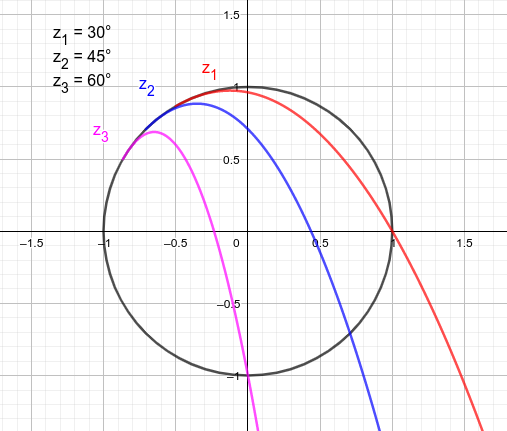
\includegraphics[scale=0.75]{Bahnkurve}
		\end{align*}
	\end{enumerate}

\end{document}